\documentclass[a4paper]{report}
\usepackage[utf8]{inputenc}
\usepackage{amsmath,amssymb,amsfonts,amsthm,stmaryrd}
\usepackage{mathrsfs} % per mathscr
\usepackage{dsfont} % per mathbb1
\usepackage{graphicx}% ruota freccia per le azioni
\usepackage{oldgerm} % Fractur Particolare
\usepackage{marvosym}% per il \Lightning
\usepackage{array}
\usepackage{faktor} %per gli insiemi quoziente
\usepackage{hyperref}
\usepackage{xparse} % Per nuovi comandi con tanti input opzionali
\usepackage{tikz-cd}
\usepackage{multicol}
\usepackage{multirow}
\usepackage{cancel}

%\usepackage[italian]{babel}
\usepackage[position=top]{subfig}
\usepackage{setspace}
\usepackage{mdframed}
\usepackage{calc}
\usepackage{enumerate}
\usepackage{centernot}
\usepackage{comment}

\usepackage{ mathdots }

% Ambienti per teoremi =================================
% <name> 
% <space above> 
% <space below> 
% <body font> 
% <indent amount> 
% <Theorem head font> 
% <punctuation after theorem head> 
% <space after theorem head> (default .5em) 
% <Theorem head spec>

% I nuovi ambienti sono costruiti in modo da andare alla riga successiva

\newsavebox{\boiteencadrement}
\newenvironment{encadrement}[1][gray!15]
  {\par\addvspace{\topsep+10pt}%
   \def\couleurencadrement{#1}%
   \begin{lrbox}{\boiteencadrement}%
   \begin{minipage}{\linewidth-6\fboxsep-1pt}%
  }
  {\end{minipage}\end{lrbox}%
   \noindent
\begin{tikzpicture}[
   inner sep=8pt,
   line width=0.75pt]
   \node[rounded corners = 5pt,
   draw,
   color=black,
   fill=\couleurencadrement] {\usebox{\boiteencadrement}};
   \end{tikzpicture}%
   \par\addvspace{\topsep+10pt}%
  }

%Equazioni
\numberwithin{equation}{section} 

%Teoremi
\theoremstyle{plain}

%\newtheorem{lem}[thm]{Lemma}
%\newtheorem{exer}[thm]{Esercizio}
%\newtheorem{cor}[thm]{Corollary}

\theoremstyle{definition}

\newcounter{theorem}
\counterwithin{theorem}{chapter}

    %thm
\newtheorem{pretrm}[theorem]{Theorem}
\newenvironment{theorem}{\begin{encadrement}\begin{pretrm}}{\end{pretrm}\end{encadrement}}

\newtheorem{prefct}[theorem]{Fact}
\newenvironment{fact}{\begin{encadrement}\begin{prefct}}{\end{prefct}\end{encadrement}}

%\newtheorem{definition}[theorem]{Definition}
%\newcounter{definition}
    %def
\newtheorem{predef}[theorem]{Definition}
\newenvironment{definition}{\begin{encadrement}\begin{predef}}{\end{predef}\end{encadrement}}
    %prop
\newtheorem{preprop}[theorem]{Proposition}
\newenvironment{proposition}{\begin{encadrement}\begin{preprop}}{\end{preprop}\end{encadrement}}
    %cor
\newtheorem{precor}[theorem]{Corollary}
\newenvironment{corollary}{\begin{encadrement}\begin{precor}}
{\end{precor}\end{encadrement}}
    %lem
\newtheorem{prelem}[theorem]{Lemma}
\newenvironment{lemma}{\begin{encadrement}\begin{prelem}}{\end{prelem}\end{encadrement}}
%
\newtheorem{conjecture}[theorem]{Conjecture}
\newtheorem{example}[theorem]{Example}
\newtheorem{exercise}[theorem]{Exercise}
\newtheorem{remark}[theorem]{Remark}
\newtheorem*{notation}{Notation}

\makeatletter
\renewenvironment{proof}[1][\proofname]
{
    \par
    \pushQED{\qed}
    \normalfont \topsep6\p@\@plus6\p@\relax
    \trivlist
    \item[\hskip\labelsep\itshape#1\@addpunct{.}]\mbox{}\\*
}
{
    \popQED\endtrivlist\@endpefalse
}
\makeatother



%========= Preambolo per quiver ================
% quiver e' uno strumento che uso spesso per
% disegnare diagrammi. L'interfaccia sul loro sito
% permette di creare in modo visivo il diagramma e
% poi esportarlo come codice LaTeX da inserire nel
% documento. Il sito e' https://q.uiver.app/ 

%-----------------------------------------------
% *** quiver ***
% A package for drawing commutative diagrams exported from https://q.uiver.app.
%
% This package is currently a wrapper around the `tikz-cd` package, importing necessary TikZ
% libraries, and defining a new TikZ style for curves of a fixed height.
%
% Version: 1.2.1
% Authors:
% - varkor (https://github.com/varkor)
% - Andr\e'C (https://tex.stackexchange.com/users/138900/andr%C3%A9c)

\NeedsTeXFormat{LaTeX2e}
%\ProvidesPackage{quiver}[2021/01/11 quiver]

% `tikz-cd` is necessary to draw commutative diagrams.
\RequirePackage{tikz-cd}
% `amssymb` is necessary for `\lrcorner` and `\ulcorner`.
\RequirePackage{amssymb}
% `calc` is necessary to draw curved arrows.
\usetikzlibrary{calc}
% `pathmorphing` is necessary to draw squiggly arrows.
\usetikzlibrary{decorations.pathmorphing}

% A TikZ style for curved arrows of a fixed height, due to Andr\e'C.
\tikzset{curve/.style={settings={#1},to path={(\tikztostart)
    .. controls ($(\tikztostart)!\pv{pos}!(\tikztotarget)!\pv{height}!270:(\tikztotarget)$)
    and ($(\tikztostart)!1-\pv{pos}!(\tikztotarget)!\pv{height}!270:(\tikztotarget)$)
    .. (\tikztotarget)\tikztonodes}},
    settings/.code={\tikzset{quiver/.cd,#1}
        \def\pv##1{\pgfkeysvalueof{/tikz/quiver/##1}}},
    quiver/.cd,pos/.initial=0.35,height/.initial=0}

% TikZ arrowhead/tail styles.
\tikzset{tail reversed/.code={\pgfsetarrowsstart{tikzcd to}}}
\tikzset{2tail/.code={\pgfsetarrowsstart{Implies[reversed]}}}
\tikzset{2tail reversed/.code={\pgfsetarrowsstart{Implies}}}
% TikZ arrow styles.
\tikzset{no body/.style={/tikz/dash pattern=on 0 off 1mm}}
%=================================================

%PER CAMBIARE I MARGINI
\usepackage[margin=4cm]{geometry}

%\usepackage{emptypage} % Pagine vuote non numerate
%\usepackage{fancyhdr} % Sistema headers
%\usepackage[Lenny]{fncychap} % Capitoli fighi
%\ChTitleVar{\Huge\bfseries}
\usepackage[hang,flushmargin]{footmisc} % Footnote non indentata


%========== Stile header e footer ==============

%\pagestyle{fancy}
% Left, Right, Even(pages), Odd(pages), Center
%\fancyhead[L]{\leftmark}
%\fancyfoot[C]{}

%\renewcommand{\chaptermark}[1]{\markboth{\textsc{#1}}{}}
%\renewcommand{\sectionmark}[1]{\markright{\textsc{#1}}}

%\renewcommand{\headrulewidth}{0.05pt}
%\renewcommand{\footnoterule}{\kern 0pt	\hrule width \textwidth height 0.5pt \kern 5pt}

%Numeri pagina in prima pagina capitoli
%\makeatletter
%\let\ps@plain\ps@empty
%\makeatother

%==== Colore dei footnote, link e citazioni ====
\definecolor{DarkBlue}{HTML}{00518B}
\definecolor{DarkRed}{HTML}{B6321C}
\hypersetup{
    colorlinks=true,
    linkcolor=DarkRed,
    filecolor=blue,
    citecolor = DarkRed,
    urlcolor=cyan,
}
\renewcommand\thefootnote{\textcolor{blue}{\arabic{footnote}}}
%============ Simboli standard =================
%----------------- Lettere ---------------------
\newcommand{\A}{\mathbb{A}}
\newcommand{\B}{\mathbb{B}}
\newcommand{\C}{\mathbb{C}}
\newcommand{\D}{\mathbb{D}}
\newcommand{\E}{\mathbb{E}}
\newcommand{\F}{\mathbb{F}}
\newcommand{\G}{\mathbb{G}}
\newcommand{\Hb}{\mathbb{H}}
\newcommand{\I}{\mathbb{I}}
\newcommand{\J}{\mathbb{J}}
\newcommand{\K}{\mathbb{K}}
\newcommand{\Lb}{\mathbb{L}}
\newcommand{\M}{\mathbb{M}}
\newcommand{\N}{\mathbb{N}}
\newcommand{\Ob}{\mathbb{O}}
\newcommand{\Pj}{\mathbb{P}}
\newcommand{\Q}{\mathbb{Q}}
\newcommand{\R}{\mathbb{R}}
\newcommand{\Sb}{\mathbb{S}}
\newcommand{\T}{\mathbb{T}}
\newcommand{\U}{\mathbb{U}}
\newcommand{\V}{\mathbb{V}}
\newcommand{\W}{\mathbb{W}}
\newcommand{\X}{\mathbb{X}}
\newcommand{\Y}{\mathbb{Y}}
\newcommand{\Z}{\mathbb{Z}}

\newcommand{\Ac}{\mathcal{A}}
\newcommand{\Bc}{\mathcal{B}}
\newcommand{\Cc}{\mathcal{C}}
\newcommand{\Dc}{\mathcal{D}}
\newcommand{\Ec}{\mathcal{E}}
\newcommand{\Fc}{\mathcal{F}}
\newcommand{\Gc}{\mathcal{G}}
\newcommand{\Hc}{\mathcal{H}}
\newcommand{\Ic}{\mathcal{I}}
\newcommand{\Jc}{\mathcal{J}}
\newcommand{\Kc}{\mathcal{K}}
\newcommand{\Lc}{\mathcal{L}}
\newcommand{\Mc}{\mathcal{M}}
\newcommand{\Nc}{\mathcal{N}}
\newcommand{\Oc}{\mathcal{O}}
\newcommand{\Pc}{\mathcal{P}}
\newcommand{\Qc}{\mathcal{Q}}
\newcommand{\Rc}{\mathcal{R}}
\newcommand{\Sc}{\mathcal{S}}
\newcommand{\Tc}{\mathcal{T}}
\newcommand{\Uc}{\mathcal{U}}
\newcommand{\Vc}{\mathcal{V}}
\newcommand{\Wc}{\mathcal{W}}
\newcommand{\Xc}{\mathcal{X}}
\newcommand{\Yc}{\mathcal{Y}}
\newcommand{\Zc}{\mathcal{Z}}

\newcommand{\Af}{\mathfrak{A}}
\newcommand{\Bf}{\mathfrak{B}}
\newcommand{\Cf}{\mathfrak{C}}
\newcommand{\Df}{\mathfrak{D}}
\newcommand{\Ef}{\mathfrak{E}}
\newcommand{\Ff}{\mathfrak{F}}
\newcommand{\Gf}{\mathfrak{G}}
\newcommand{\Hf}{\mathfrak{H}}
\newcommand{\If}{\mathfrak{I}}
\newcommand{\Jf}{\mathfrak{J}}
\newcommand{\Kf}{\mathfrak{K}}
\newcommand{\Lf}{\mathfrak{L}}
\newcommand{\Mf}{\mathfrak{M}}
\newcommand{\Nf}{\mathfrak{N}}
\newcommand{\Of}{\mathfrak{O}}
\newcommand{\Pf}{\mathfrak{P}}
\newcommand{\Qf}{\mathfrak{Q}}
\newcommand{\Rf}{\mathfrak{R}}
\newcommand{\Sf}{\mathfrak{S}}
\newcommand{\Tf}{\mathfrak{T}}
\newcommand{\Uf}{\mathfrak{U}}
\newcommand{\Vf}{\mathfrak{V}}
\newcommand{\Wf}{\mathfrak{W}}
\newcommand{\Xf}{\mathfrak{X}}
\newcommand{\Yf}{\mathfrak{Y}}
\newcommand{\Zf}{\mathfrak{Z}}

\newcommand{\af}{\mathfrak{a}}

\newcommand{\cf}{\mathfrak{c}}
\newcommand{\df}{\mathfrak{d}}
\newcommand{\ef}{\mathfrak{e}}
\newcommand{\ff}{\mathfrak{f}}
\newcommand{\gf}{\mathfrak{g}}
\newcommand{\hf}{\mathfrak{h}}

\newcommand{\jf}{\mathfrak{j}}
\newcommand{\kf}{\mathfrak{k}}
\newcommand{\lf}{\mathfrak{l}}
\newcommand{\mf}{\mathfrak{m}}
\newcommand{\nf}{\mathfrak{n}}
\newcommand{\of}{\mathfrak{o}}
\newcommand{\pf}{\mathfrak{p}}
\newcommand{\qf}{\mathfrak{q}}
\newcommand{\rf}{\mathfrak{r}}

\newcommand{\tf}{\mathfrak{t}}
\newcommand{\uf}{\mathfrak{u}}
\newcommand{\vf}{\mathfrak{v}}
\newcommand{\wf}{\mathfrak{w}}
\newcommand{\xf}{\mathfrak{x}}
\newcommand{\yf}{\mathfrak{y}}
\newcommand{\zf}{\mathfrak{z}}

\newcommand{\As}{\mathscr{A}}
\newcommand{\Bs}{\mathscr{B}}
\newcommand{\Cs}{\mathscr{C}}
\newcommand{\Ds}{\mathscr{D}}
\newcommand{\Es}{\mathscr{E}}
\newcommand{\Fs}{\mathscr{F}}
\newcommand{\Gs}{\mathscr{G}}
\newcommand{\Hs}{\mathscr{H}}
\newcommand{\Is}{\mathscr{I}}
\newcommand{\Js}{\mathscr{J}}
\newcommand{\Ks}{\mathscr{K}}
\newcommand{\Ls}{\mathscr{L}}
\newcommand{\Ms}{\mathscr{M}}
\newcommand{\Ns}{\mathscr{N}}
\newcommand{\Os}{\mathscr{O}}
\newcommand{\Ps}{\mathscr{P}}
\newcommand{\Qs}{\mathscr{Q}}
\newcommand{\Rs}{\mathscr{R}}
\newcommand{\Ss}{\mathscr{S}}
\newcommand{\Ts}{\mathscr{T}}
\newcommand{\Us}{\mathscr{U}}
\newcommand{\Vs}{\mathscr{V}}
\newcommand{\Ws}{\mathscr{W}}
\newcommand{\Xs}{\mathscr{X}}
\newcommand{\Ys}{\mathscr{Y}}
\newcommand{\Zs}{\mathscr{Z}}

\newcommand{\ula}{{\underline{a}}}
\newcommand{\ulb}{{\underline{b}}}
\newcommand{\ulc}{{\underline{c}}}
\newcommand{\uld}{{\underline{d}}}
\newcommand{\ule}{{\underline{e}}}
\newcommand{\ulf}{{\underline{f}}}
\newcommand{\ulg}{{\underline{g}}}
\newcommand{\ulh}{{\underline{h}}}
\newcommand{\uli}{{\underline{i}}}
\newcommand{\ulj}{{\underline{j}}}
\newcommand{\ulk}{{\underline{k}}}
\newcommand{\ull}{{\underline{l}}}
\newcommand{\ulm}{{\underline{m}}}
\newcommand{\uln}{{\underline{n}}}
\newcommand{\ulo}{{\underline{o}}}
\newcommand{\ulp}{{\underline{p}}}
\newcommand{\ulq}{{\underline{q}}}
\newcommand{\ulr}{{\underline{r}}}
\newcommand{\uls}{{\underline{s}}}
\newcommand{\ult}{{\underline{t}}}
\newcommand{\ulu}{{\underline{u}}}
\newcommand{\ulv}{{\underline{v}}}
\newcommand{\ulw}{{\underline{w}}}
\newcommand{\ulx}{{\underline{x}}}
\newcommand{\uly}{{\underline{y}}}
\newcommand{\ulz}{{\underline{z}}}

%---------- Funzioni standard ------------------
\DeclareMathOperator{\Adj}{Adj}
\DeclareMathOperator{\adj}{adj}
\DeclareMathOperator{\Ann}{Ann}
\DeclareMathOperator{\Arg}{Arg}
\DeclareMathOperator{\Ass}{Ass}
\DeclareMathOperator{\cha}{char}
\DeclareMathOperator{\cod}{cod}
\DeclareMathOperator{\coker}{coker}
\DeclareMathOperator{\comb}{Comb}
\DeclareMathOperator{\dom}{dom}
\DeclareMathOperator{\End}{End}
\DeclareMathOperator{\Fix}{Fix}
\DeclareMathOperator{\Frac}{Frac}
\DeclareMathOperator{\Hom}{Hom}
\DeclareMathOperator{\imm}{Imm}
\DeclareMathOperator{\Ind}{Ind}
\DeclareMathOperator*{\infess}{infess}
\DeclareMathOperator{\mcd}{mcd}
\DeclareMathOperator{\mcm}{mcm}
\DeclareMathOperator{\Min}{Min}
\DeclareMathOperator{\Mor}{Mor}
\DeclareMathOperator{\obj}{obj}
\DeclareMathOperator{\orb}{orb}
\DeclareMathOperator{\ord}{ord}
\DeclareMathOperator{\Proj}{Proj}
\DeclareMathOperator{\Res}{Res}
\DeclareMathOperator{\rnk}{rnk}
\DeclareMathOperator{\sgn}{sgn}
\DeclareMathOperator{\Span}{Span}
\DeclareMathOperator{\Spec}{Spec}
\DeclareMathOperator{\stab}{stab}
\DeclareMathOperator*{\supess}{supess}
\DeclareMathOperator{\Supp}{Supp}
\DeclareMathOperator{\supp}{supp}
\DeclareMathOperator{\Sym}{Sym}
\DeclareMathOperator{\tr}{tr}

\newcommand{\Real}{\,\Re\mathfrak{e}}
\newcommand{\Imag}{\,\Im\mathfrak{m}}



%-------------- Frecce -------------------------
\newcommand{\coimplies}{\Longleftrightarrow}
\newcommand{\inj}{\hookrightarrow}
\newcommand{\onto}{\twoheadrightarrow}
\newcommand{\ot}{\leftarrow}
\newcommand{\acts}{\curvearrowright}

%----------- Lettere greche -------------------
\newcommand{\al}{\alpha}
\newcommand{\de}{\delta}
\newcommand{\e}{\varepsilon}
%\newcommand{\th}{\theta}
\newcommand{\la}{\lambda}
\newcommand{\vp}{\varphi}

%-------------- Derivate ----------------------
\newcommand{\raiseargument}[1]{\raisebox{.8ex}{$#1$}}
\newcommand{\centersmallmath}[1]{\vcenter{\hbox{\scalebox{.8}{$#1$}}}}
\newcommand{\raiseargumentsmall}[1]{\raisebox{.4ex}{\scalebox{.8}{$#1$}}}
\newcommand*{\emptyfrac}[2]{\genfrac{}{}{0pt}{}{#1}{#2}}

\NewDocumentCommand{\ddxi}{O{x}mm}{
    {\frac{d^{}{#3}}{d{#1}_{#2}}}
}

\NewDocumentCommand{\dd}{O{}mm}{
    {\frac{d^{#1}{#3}}{d{#2}^{#1}}}
}

\NewDocumentCommand{\ppxi}{O{x}mm}{
    {{\frac{\partial^{}{#3}}{\partial{#1}_{#2}}}}
}

\NewDocumentCommand{\pp}{O{}mm}{
    {{\frac{\partial^{#1}{#3}}{\partial{#2}}}}
}





%========== Comandi dattilografici ============
%--------- Passaggi in derivazioni ------------
\newcommand{\pasg}[3]{\overset{\hyperref[#3]{\text{#2}}}{#1}}
\newcommand{\pasgnl}[2]{\overset{\text{#2}}{#1}}
\newcommand{\pasgnlmath}[2]{\overset{#2}{#1}}
\newcommand{\pasgmath}[3]{\overset{\hyperref[#3]{{#2}}}{#1}}

%----------- Modifica testo -------------------
\newcommand{\ul}[1]{\underline{#1}}
\newcommand{\ol}[1]{\overline{#1}}
\newcommand{\wt}[1]{\widetilde{#1}}
\newcommand{\wh}[1]{\widehat{#1}}
\newcommand{\td}[1]{\Tilde{#1}}
\newcommand{\rg}[1]{{\mathring {#1}}}
\newcommand{\under}[2]{\underset{#1}{\underbrace{#2}}}

%-------------- Parentesi ---------------------
\newcommand{\pa}[1]{\left({#1}\right)}
\newcommand{\spa}[1]{\left[{#1}\right]}
\newcommand{\cpa}[1]{\left\{{#1}\right\}}
\newcommand{\abs}[1]{\left|{#1}\right|}
\newcommand{\norm}[1]{\left\Vert{#1}\right\Vert}
\newcommand{\ps}[1]{\left\langle {#1}\right\rangle}
\newcommand{\floor}[1]{\left\lfloor {#1}\right\rfloor}
\newcommand{\ceil}[1]{\left\lceil {#1}\right\rceil}
\newcommand{\rbar}[1]{\left.{#1}\right|}

%--------------- Matrici ----------------------
\newcommand{\mat}[1]{\begin{pmatrix}#1\end{pmatrix}}
\newcommand{\emat}[1]{\begin{matrix}#1\end{matrix}}
\newcommand{\dmat}[1]{\begin{vmatrix}#1\end{vmatrix}}
\newcommand{\smat}[1]{\begin{smallmatrix}#1\end{smallmatrix}}
\newcommand{\BIG}[1]{\mathlarger{\mathlarger{\mathlarger{\mathlarger{#1}}}}}

%--------------- Funzioni ---------------------
\newcommand{\funcDef}[4]{
\begin{array}{ccc}
{#1} & \longrightarrow & {#2}\\
{#3} & \longmapsto & {#4}
\end{array}}
\newcommand{\functorDef}[6]{
\begin{array}{ccc}
{#1} & \longrightarrow & {#2}\\
{#3} & \longmapsto & {#4}\\
{#5} & \longmapsto & {#6}
\end{array}}
\newcommand{\correspDef}[6]{
\begin{array}{ccc}
{#1} & \longleftrightarrow & {#2}\\
{#3} & \longmapsto & {#4}\\
{#5} & \longmapsfrom & {#6}
\end{array}}

%---------------- Altro -----------------------
\newcommand{\bs}{\setminus}
\newcommand{\res}[1]{\raisebox{-.5ex}{$|$}_{#1}}
\newcommand{\quot}[2]{\faktor{#1}{#2}}
\newcommand{\sep}{\,\middle|\,}

\newcommand{\ii}{^{-1}}
\newcommand{\nz}{\bs\{0\}}

\newcommand{\powerset}{\mathscr{P}}
\newcommand{\del}{\partial}
\newcommand{\0}{{\underline{0}}}
\newcommand{\1}{{\vcenter{\hbox{\scalebox{1.2}{$\mathds{1}$}}}}}
\newcommand{\bw}{\bigwedge}


\newcommand{\GL}{\mathrm{GL}}
\newcommand{\PGL}{\mathrm{PGL}}
\newcommand{\SL}{\mathrm{SL}}
%\NewDocumentCommand{\PGL}{o m}{
%    \IfNoValueTF{#1}
%        {{\mathbb{P}GL({#2})}}
%    {{\mathbb{P}GL_{#1}({#2})}}
%}
%\NewDocumentCommand{\GL}{o m}{
%    \IfNoValueTF{#1}
%        {{GL({#2})}}
%    {{GL_{#1}({#2})}}
%}
\newcommand{\znz}[1]{{\Z/{#1}\Z}}







\usepackage{cleveref}


% ============================================


%---------- Comandi specifici ----------------
\DeclareMathOperator{\Der}{Der}
\DeclareMathOperator{\SO}{SO}
\DeclareMathOperator{\Mat}{Mat}
\DeclareMathOperator{\Fun}{Fun}

\newcommand{\Diag}{\mathrm{Diag}}
\newcommand{\Ab}{\mathrm{Ab}}
\newcommand{\Mon}{\mathrm{Mon}}

\newcommand{\op}{^{op}}

%--------- Comandi dattilografici ------------
\newcommand{\coloneqq}{:=}


% ============================================
\title{\huge Toric Varieties - Geometria Algebrica F
\vspace{0.7cm}

\Large Corso del prof. Talpo Mattia}

\author{\Large Francesco Sorce}
\date{Università di Pisa\\
Dipartimento di Matematica\\
A.A. 2024/25}

\begin{document}
\maketitle

%\newpage
\tableofcontents
\newpage

\chapter*{Introduction}
\section*{Syllabus}
The first part of the course deals with:
\begin{itemize}
    \item Algebraic Tori, their actions and representations
    \item Affine toric varieties (with monoids) $\leftrightarrow$ cones in some $\R^n$
    \item Projective toric varieties $\leftrightarrow$ polytopes in some $\R^n$
    \item General toric varieties $\leftrightarrow$ fans in $\R^n$
\end{itemize}
We will then deal with (subject to change)
\begin{itemize}
    \item Divisors/line bundles on toric varieties
    \item Cox ring of a toric variety
    \item Cohomology of divisors
    \item Toric morphisms and resolution of singularities
    \item and more...?
\end{itemize}
The main reference for this course \textemdash ``Toric varieties" by Cox, Little, Schenck \cite{cox2011toric} \textemdash is available in the same folder as this PDF.

\section*{What is the course about?}
We will work over an algebraically closed field (and we will be lax about the characteristic of the field). In \cite{cox2011toric} the authors work over $\C$ but many results hold more generally.
\medskip

The main goal of the course is understanding toric varieties:
\begin{definition}[Toric variety]
An $n$-dimensional toric variety $X$ is a (normal) $k$-variety equipped with an open immersion of an $n$-dimensional torus $T\subseteq X$, where $T\cong (k^\ast)^n$, and an action $T\times T\to T$ which extends to the whole of $X$ \footnote{that is, it extends to a $T\times X\to X$}.
\end{definition}

\begin{remark}
Normality is a standard assumption that we'll make at some point but some things work without it.
\end{remark}

We'll see that the geometry of such an object is encoded in a combinatorial gadget, converting problems in algebraic geometry to problems in combinatorics, which is sometimes convenient.

The opposite reduction is also possible and has been used historically. One of the main examples of a combinatorial problem being solved via the geometry of toric varieties is
\begin{example}[McMullen's ``$g$-conjecture"]

The then conjecture, and now theorem, is a characterization of the $f$-vectors of simple polytopes\footnote{for now a simple polytope is the convex hull of a finite subset of $\R^n$}.

\begin{definition}[$f$-vectors]
If $P$ is a polytope, its \textbf{$f$-vector} is 
\[(f_0(P),\cdots, f_d(P)),\quad \text{where $d=\dim P$}\]
and $f_i(P)$ is the number of $i$-dimensional faces. We may set $f_{-1}(P)=1$.
\end{definition}

It's reasonable to ask ourselves which $f$-vectors can appear. We may define the \textbf{$h$-vector} by setting
\[\sum_{i=0}^d f_i (t-1)^i=\sum_{i=0}^dh_i t^i,\quad \text{i.e. }h_i=\sum_{j=i}^d(-1)^{j-i}\binom{j}if_j,\ h_{-1}=0.\]
It was a known theorem that the $h$-vector of a simple polytope is palindromic (i.e. $h_i=h_{d-i}$).
From the $h$-vector we obtain the \textbf{$g$-vector} by setting $g_i=h_i-h_{i-1}$. 

The conjecture was that
\begin{theorem}[$g$-conjecture]
$f=(f_0,\cdots, f_d)\in \N^{d+1}$ is the $f$-vector of a simple polytope if
\begin{enumerate}
\item $h_i=h_{d-1}$ for all $0\leq i\leq \floor{d/2}$
\item $g_i\geq 0$ for all $0\leq i\leq \floor{d/2}$
\item $(g_1,\cdots, g_{\floor{d/2}})$ is a ``Macauly vector" if, when we write (uniquely)
\[g_i=\binom{n_i}i+\cdots+\binom{n_{r_i}}{r_i}\]
with $n_i>n_{i-1}>\cdots>n_{r_i}$ then
\[g_{i+1}\leq \binom{n_i+1}{i+1}+\cdots+\binom{n_{r_i}+1}{r_i+1}\]
\end{enumerate}
\end{theorem}
Stanley proved necessity using toric varieties. He proved that the $g$-vector of a simple polytope is the vector of dimensions for some cohomology ring of the associated toric variety.


Later McMullen found a completely combinatorial proof but for some time the only proof of this combinatorial fact passed through the geometry of toric varieties.
\end{example}

\part{Basic theory of toric varieties}
\chapter{Algebraic tori and their actions}

\section{Basic definitions}
\begin{definition}[Algebraic group]
An \textbf{algebraic group} $G$ is a $k$-variety equipped with the the structure of a ``group object" in the category of $k$-varieties, i.e. we have two morphisms and a \textit{closed} point
\[m:G\times G\to G,\quad i:G\to G,\quad e\in G\]
that satisfy the usual group axioms ``diagrammatically".
\end{definition}

\begin{example}
Associativity can be expressed ``diagrammatically" as
% https://q.uiver.app/#q=WzAsNCxbMCwwLCJHXFx0aW1lcyBHXFx0aW1lcyBHIl0sWzEsMCwiR1xcdGltZXMgRyJdLFswLDEsIkdcXHRpbWVzIEciXSxbMSwxLCJHIl0sWzAsMiwiKG0saWRfRykiLDJdLFswLDEsIihpZF9HLG0pIl0sWzEsMywibSJdLFsyLDMsIm0iLDJdXQ==
\[\begin{tikzcd}
	{G\times G\times G} & {G\times G} \\
	{G\times G} & G
	\arrow["{(id_G,m)}", from=1-1, to=1-2]
	\arrow["{(m,id_G)}"', from=1-1, to=2-1]
	\arrow["m", from=1-2, to=2-2]
	\arrow["m"', from=2-1, to=2-2]
\end{tikzcd}\]
\end{example}

\begin{definition}[Multiplicative group]
The \textbf{multiplicative group}, denoted $\G_m$, is the $k$-variety $\A^1\bs \cpa0$ equipped with the morphisms
\[m:\funcDef{\G_m\times \G_m}{\G_m}{(a,b)}{ab}\]
\[i:\funcDef{\G_m}{\G_m}{a}{1/a}\]
\[e=1\in \A^1\nz\]
(we are identifying $\G_m=k^\ast$).
\end{definition}

\begin{remark}
$\G_m$ is affine: $\A^1=\Spec k[x]$ and $\A^1\nz=\A^1\bs V(x)=D(x)$, thus $D(x)=\Spec (k[x])_{x}=\Spec(k[x,x\ii])=\Spec k[x^{\pm1}]$.
\end{remark}

\begin{remark}
All affine algebraic groups can be described dually as spectra of \textbf{Hopf algebras}
\end{remark}


\begin{example}
$m:\G_m\times \G_m\to \G_m$ can be described as the map corresponding to
\[\funcDef{k[x^{\pm1}]}{k[y^{\pm1}]\otimes_k k[z^{\pm1}]}{x}{y\otimes z}\]
the inverse corresponds to
\[\funcDef{k[x^{\pm1}]}{k[y^{\pm1}]}{x}{y\ii}\]
and the neutral element corresponds to\footnote{recall that a $k$-point $e$ of the variety $G$ can be seen as a morphism $\Spec k\to G$ with set-theoretic image $e$.}
\[\funcDef{k[x^{\pm1}]}{k}{x}{1}\]
\end{example}

\begin{remark}
In general, if $G=\Spec A$ is an affine variety, a structure of algebraic group is equivalent to a structure of Hopf algebra on $A$:
\begin{align*}
m:G\times G\to G\quad\longleftrightarrow& \quad\Delta:A\to A\otimes_k A\\
i:G\to G\quad\longleftrightarrow& \quad S:A\to  A\\
e:\Spec k\to G\quad\longleftrightarrow& \quad\e:A\to k
\end{align*}
\end{remark}

\begin{remark}
If $G$ and $H$ are algebraic groups, $G\times H$ is also naturally an alegbraic group.
\end{remark}

\begin{definition}[Algebraic tori]
The \textbf{standard $n$-dimensional algebraic torus over $k$} is $\G_m^n$. An \textbf{algebraic torus} is an algebraic groups $T$ which is isomorphic to $\G_m^n$ for some $n$.

We may omit the adjective ``algebraic" when appropriate.
\end{definition}

\begin{remark}
If $k=\C$ then $\G_m^n=(\C^\ast)^n$, which is homotopy equivalent to $(S^1)^n$. This $(S^1)^n$ is the ``maximal compact subgroup".
\end{remark}


\section{Cartier duality}

In some sense which we will make precise, tori are ``dual" to finitely generated torsion-free (and thus free) abelian groups.

\begin{definition}[Associated group algebra]
If $M$ is a finitely generated abelian group, the \textbf{$k$-group algebra of $M$}, denoted by $k[M]$, is the freely generated $k$-vector space with formal basis $\cpa{t^m\mid m\in M}$ and multiplication induced by $t^mt^{m'}=t^{m+m'}$.
\end{definition}

\begin{example}
If $M=\Z^n$ then
\[k[\Z^n]=k[x_1^{\pm1},\cdots,x_n^{\pm1}],\]
which is the coordinate ring of $(\G_m)^n$.

Moreover, the group structure of $\G_m^n$ is given by
\begin{align*}
\Delta:&\funcDef{k[\Z^n]}{k[\Z^n]\otimes_k[\Z^n]}{t^m}{t^m\otimes t^m}\\
S:&\funcDef{k[\Z^n]}{k[\Z^n]}{t^m}{t^{-m}}\\
\e:&\funcDef{k[\Z^n]}{k}{t^m}{1}
\end{align*}
\end{example}

\begin{fact}
These formulas give a Hopf algebra structure on $k[M]$ for all abelian groups $M$
\begin{align*}
\Delta:&\funcDef{k[M]}{k[M]\otimes_k[M]}{t^m}{t^m\otimes t^m}\\
S:&\funcDef{k[M]}{k[M]}{t^m}{t^{-m}}\\
\e:&\funcDef{k[M]}{k}{t^m}{1}
\end{align*}
\end{fact}

\begin{remark}
$k[M]$ is finitely generated and reduced, so there is a (classical) affine variety $D(M):=\Spec k[M]$ which inherits the structure of an algebraic group.
\end{remark}


\begin{definition}[Cartier dual]
If $M$ is a finitely generated abelian group, $D(M)$ is the \textbf{cartier dual} of $M$.
\end{definition}

\begin{example}
If $M=\znz n$ then the group algebra is
\[k[\znz n]=\frac{k[t]}{(t^n-1)}.\]
$\Spec k[\znz n]$ then is the closed subvariety (and subgroup) of $\G_m$ described by the equation $t^n=1$, i.e. the group of the $n$-th roots of unity $\mu_n$
\end{example}

\begin{definition}[Group of $n$-th roots of unity]
$\mu_n=D(\znz n)$.
\end{definition}

\begin{remark}
If $n=p=\cha k$ then $(t^p-1)=(t-1)^p$, so $\mu_p$ would be a point. To get any interesting geometric information in this case you need to allow nilpotens and you end up with a group scheme.
\end{remark}


\begin{exercise}
$D(M\oplus N)=D(M)\times D(N)$.
\end{exercise}

For a general finitely generated abelian group
\[M=\Z^n\oplus \znz{n_1}\oplus\cdots\oplus \znz{n_k}\]
we get
\[D(M)\cong \G_m^n\times\mu_{n_1}\times\cdots\times\mu_{n_k}.\]


\begin{remark}
$\GL_n$ is an algebraic group, indeed $\GL_n\subseteq \A^{n^2}$ and we can give it the structure of a variety by seeing it as the principal open subset associated to the determinant (seen as a regular function on $\A^{n^2}$). Matrix multiplication and inversion can be checked to be morphisms.
\end{remark}

\begin{definition}[Diagonizable group]
An algebraic group is called \textbf{diagonalizable} if it is isomorphic to a (closed) subgroup of $\Diag_n\subseteq \GL_n$ for some $n$
\end{definition}

\begin{remark}
$\Diag_n\cong\G_m^n$
\end{remark}

\begin{fact}
We have an equivalence of categories
\[D:(fin.gen.AbGps)\to (Diagonalizable.AlgGroups)\]
\end{fact}




\chapter{Affine toric varieties}

\section{Introduction}

\begin{definition}[Affine toric variety]
An \textbf{affine toric variety} is an irreducible affine variety $X$ equipped with an open embedding of a torus $T$ such that the translation action $T\times T\to T$ extends to an action of $T$ on $X$.
\end{definition}

\begin{remark}
The open torus is automatically dense in, and of the same dimension of, $X$.
\end{remark}

\begin{remark}
The extension of the action is unique because if $X$ and $Y$ are irreducible affine and $f,g:X\to Y$ agree on a dense open subset then $f=g$.
\end{remark}

\begin{example}
A torus is a toric variety.
\end{example}

\begin{example}
Affine space $\A^n$ is a toric variety, via the trivial embedding 
\[\G_m^n=\cpa{x_1\cdots x_n\neq 0}\subseteq \A^n.\]
\end{example}

\begin{example}
Let $C=V(x^3-y^2)\subseteq \A^2$ with torus
\[\funcDef{\G_m}{C}{t}{(t^2,t^3)}\]
and action
\[\funcDef{\G_m\times C}{C}{(t,(x,y))}{(t^2x,t^3y)}.\]
Notice that this affine toric variety is neither smooth nor normal\footnote{$\Spec A$ irreducible affine variety is \textbf{normal} if all local rings are integrally closed in $\Frac A$. This is equivalent to $A$ being integrally closed in $\Frac A$.}.
\end{example}

\begin{fact}
A normal variety is smooth in codimension 1, that it, the singular locus has codimension at least 2. In particular a curve is normal iff they're smooth.
\end{fact}


\begin{example}
Let $X=V(xy-z^2)\subseteq \A^3$ be the \textit{quadric cone}. It can be shown that $X$ is normal, but it is not smooth (not at the origin).

\begin{figure}[!htb]
    \centering
    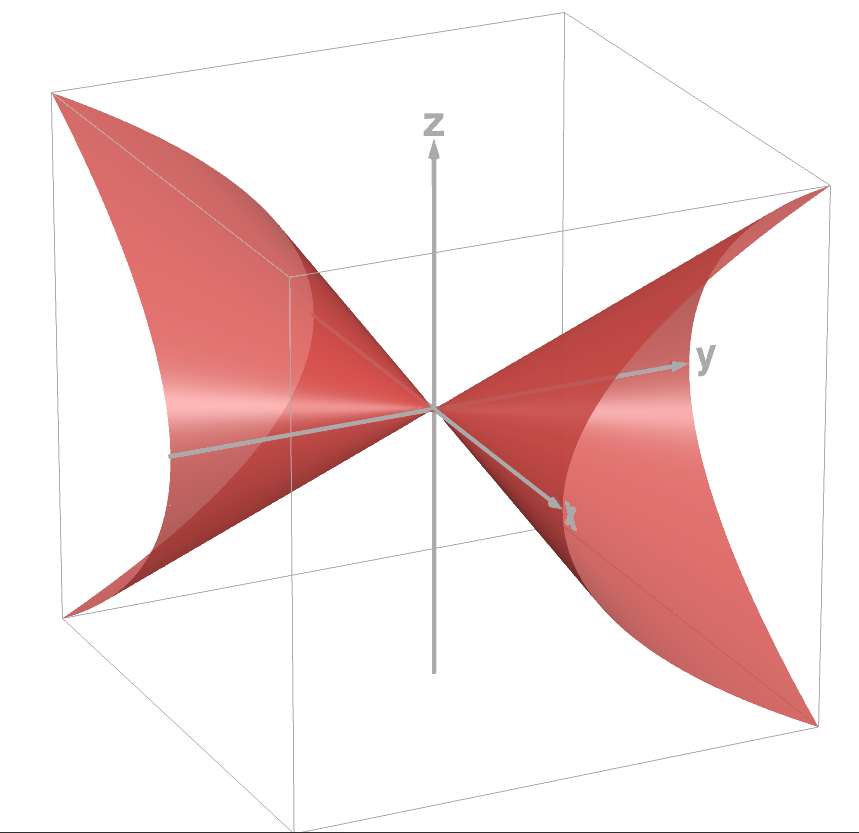
\includegraphics[width=6cm]{Images/quadric cone.png}
    \caption{Quadric cone over the real numbers.}
\end{figure}


$X$ is a toric variety with torus given by the image of\footnote{this map is 2:1, to get the actual parametrization we need
\[\funcDef{\G_m^2}{X}{(s,t)}{(s,st^2,st)}\]
This is related to the fact that $X$ is the quotient $\A^2/\mu_2$ by the action $-1(x,y)=(-x,-y)$.}
\[\funcDef{\G_m^2}{X}{(s,t)}{(s^2,t^2,st)}\]
and action
\[\funcDef{\G_m^2\times X}{X}{((s,t),(x,y,z))}{(sx,st^2y,stz)}\]
\end{example}


\begin{example}
$X=V(xy-zw)\subseteq \A^4$ is a toric variety with torus
\[\funcDef{\G_m^3}{X}{(t_1,t_2,t_3)}{(t_1,t_2,t_3,t_1t_2t_3\ii)}\]
and action 
\[\funcDef{\G_m^3\times X}{X}{((t_1,t_2,t_3),(x,y,z,w))}{(t_1x,t_2y,t_3z,t_1t_2t_3\ii w)}\]
\end{example}


\section{Monoids}

\begin{definition}[Monoid]
A \textbf{monoid} is a set $S$ with an operation $+$, which is commutative, associative and with a neutral element $0\in S$.
\end{definition}

\begin{remark}
The reference book \cite{cox2011toric} calls these \textit{semigroups}.
\end{remark}


\begin{definition}
If $A\subseteq S$ is a subset of a monoid, the \textbf{submonoid generated by $A$ in $S$} is the smallest submonoid which contains $A$. Concretely it is 
\[\ps A=\cpa{\sum_{a\in A} n_a a\mid n_a\in \N,\ n_a=0\text{ for all but finitely many coeff.}}\]
A monoid $S$ is \textbf{finitely generated} if there exists a finite subset $A\subseteq S$ such that $S=\ps A$.
\end{definition}

\begin{remark}
$S$ is a finitely generated monoid if there exists a surjective monoid homomorphism
\[\N^n\onto S.\]
\end{remark}

\begin{definition}
$S$ is an \textbf{affine monoid} if it is finitely generated and it is a submonoid of a lattice $M$.
\end{definition}

\begin{example}
$\N^k\subseteq \Z^k$ is an affine monoid.
\end{example}

\begin{example}
$\znz n$ is a monoid but it is NOT affine because a lattice can't have a submonoid with torsion.
\end{example}

\begin{example}
$\ps{(1,0),(1,1)}\subseteq \N\oplus \znz{2}$ is also not affine because of torsion.
\end{example}

\begin{definition}[Integrality]
A monoid $S$ is \textbf{integral} (or \textbf{cancellative}) if $a+b=a+c\implies b=c$.
\end{definition}

\begin{fact}
A monoid $S$ is affine if and only if $S$ is
\begin{itemize}
\item finitely generated,
\item integral and
\item torsion free.
\end{itemize}
\end{fact}

Let us now define the left adjoint to the forgetful $\Ab\to \Mon$:

\begin{definition}[Associated group]
Let $S$ be a monoid. There is an \textbf{associated abelian group} $S^{gp}$, which is the initial group with a morphism from $S$. Concretely
\[S^{gp}=\frac{\cpa{(s,s')\mid s,s'\in S}}\sim\]
where $(s_1,s'_1)\sim(s_2,s'_2)$ if there exists $s\in S$ such that\footnote{think about localization on rings which are not domains.}
\[s+s_1+s_2'=s+s_2+s_1'.\]
\end{definition}

\begin{remark}
$S^{gp}$ is an abelian group and we have a map $S\to S^{gp}$ given by $s\mapsto [(s,0)]_\sim$.
\end{remark}


\begin{fact}
Any morphism $S\to G$ for $G$ abelian group factors uniquely through $S^{gp}$. More precisely
\[\Hom_{\text{Mon}}(S,G)=\Hom_{\text{Ab}}(S^{gp},G)\]
\end{fact}


\begin{remark}
$S$ is integral if and only if $S\to S^{gp}$ is injective, which happens if and only if $S$ can be injected into an abelian group.
\end{remark}

\subsubsection{Presentations of monoids}
With monoids, the kernel is ``sort of useless"
\begin{example}
Consider
\[\funcDef{\N^2}{\N}{(a,b)}{a+b}\]
this has trivial kernel (preimage of $0$ is just $(0,0)$) but it is far from being injective.
\end{example}

Let $f:S\to S'$ be a surjective homomorphism. What we should look at instead of the kernel for the right analogue of the first isomorphism theorem is
\[E=\cpa{(s,s')\in S\times S\mid f(s)=f(s')}.\]
This set is an equivalence relation on $S\times S$, which is also a submonoid.

\begin{definition}[Congruence relations]
A submonoid of $S\times S$ which defines an equivalence relation is called \textbf{congruence relation}.
\end{definition}

\begin{definition}[Coequalizer]
If $f,g:X\to Y$, the coequalizer is an object $Z$ together with $h:Y\to Z$ such that $h\circ f=h\circ g:X\to Z$ and if $W$ together with $h':Y\to W$ is also such that $h'\circ f=c'\circ g$ then there exists a unique $Z\to W$ making everything commute.
% https://q.uiver.app/#q=WzAsNCxbMCwxLCJYIl0sWzEsMSwiWSJdLFsyLDEsIloiXSxbMiwwLCJXIl0sWzAsMSwiZiIsMCx7Im9mZnNldCI6LTF9XSxbMCwxLCJnIiwyLHsib2Zmc2V0IjoxfV0sWzEsMiwiaCIsMl0sWzEsMywiaCciXSxbMiwzLCJcXGV4aXN0cyEiLDIseyJzdHlsZSI6eyJib2R5Ijp7Im5hbWUiOiJkYXNoZWQifX19XV0=
\[\begin{tikzcd}
	&& W \\
	X & Y & Z
	\arrow["f", shift left, from=2-1, to=2-2]
	\arrow["g"', shift right, from=2-1, to=2-2]
	\arrow["{h'}", from=2-2, to=1-3]
	\arrow["h"', from=2-2, to=2-3]
	\arrow["{\exists!}"', dashed, from=2-3, to=1-3]
\end{tikzcd}\]
\end{definition}

\begin{fact}[]
We can construct quotients of $S$ by a congruence relation $E$ on $S\times S$ by setting it to be the coequalizer of $E\subseteq S\times S\rightrightarrows S$, where the arrows are the two projections from $S\times S$ to $S$.

We call this object the \textbf{quotient of $S$ by $E$} and denote it $S/E$.
\end{fact}

\begin{remark}
If $E$ is the relation constructed from $f:M\onto M'$ homomorphism of abelian groups viewed as monoids then $E=\cpa{(m,m')\in M\times M\mid f(m)=f(m')}=\cpa{(m,m')\mid m-m'\in \ker f}$. It follows that $M'\cong M/\ker f$ is a coequalizer for $E\rightrightarrows M$, so our definition makes sense.
\end{remark}


\begin{definition}[presentation of a monoid]
The monoid associated to
\[\ps{p_1,\cdots, p_r\mid a_1=b_i,\ i\in\cpa{1,\cdots, k}},\]
where $a_i,b_i,\in \ps{p_1,\cdots, p_r}_\N$, is the quotient of $\N^r$ by the congruence relation generated by the $(a_i,b_i)$ in $\N^r\times \N^r$.

A \textbf{presentation} of a monoid $S$ is an isomorphism with a monoid constructed as above.
\end{definition}





\subsection{Monoid algebra}
Since from abelian groups we costructed the group algebra and found connections to geometric objects, we want to generalize that construction to monoids.

\begin{definition}[Monoid algebra]
For a monoid $S$, its \textbf{monoid algebra} $k[S]$ is the $k$-vector space which is freely generated by $\cpa{t^s\mid s\in S}$ and with multiplication induced by the operation on $S$.
\end{definition}


\begin{remark}
In \cite{cox2011toric} they write $\chi^s$ instead of $t^s$ because they think of $S$ inside $M=X(T)$ for some torus.
\end{remark}

\begin{remark}
If $S$ is actually a group then the monoid algebra and group algebras coincide.
\end{remark}


\begin{example}
If $S=\N^n\subseteq \Z^n$ then $k[S]=k[x_1,\cdots, x_n]$.
\end{example}


\begin{proposition}
If $S$ is a monoid with presentation 
\[\ps{p_1,\cdots, p_r\mid a_i=b_i,\ 1\leq i\leq k},\] 
then
\[k[S]=\frac{k[t_1,\cdots, t_r]}{(t^{a_i}-t^{b_i})}\]
where if $a_i=\sum a_{ij}p_j$ we set $t^{a_i}=\prod t_j^{a_{ij}}$.
\end{proposition}
\begin{proof}[Sketch]
Let $R$ be the congruence relation on $\N^r$ generated by $\cpa{(a_i,b_i)}_{1\leq i\leq k}$. Since $R\rightrightarrows \N^r\to S$ is a coequalizer and $S\mapsto k[S]$ is a left adjoint ($\Hom_{\text{Mon}}(S,A)\cong \Hom_{k-\text{Alg}}(k[S],A)$) it follows that
\[k[R]\overset f{\underset g\rightrightarrows} k[\N^r]\to k[S]\] 
is a coequalizer in $k$-algebras, so $k[S]\cong k[\N^r]/I$ where $I=(f(x)-g(x)\mid x\in k[R])$.
\end{proof}



\begin{example}
Let $S=\ps{(2,0),(1,1),(0,2)}\subseteq \Z^2$. This monoid can be seen to be isomorphic to
\[\ps{p,q,r\mid p+q=2r}.\]
It follows that
\[k[S]\cong\frac{k[x,y,z]}{(xy-z^2)},\]
which is the coordinate ring of the quadric cone.
\end{example}

\begin{example}
Consider $S=\ps{2,3}\subseteq \N$, which has presentation
\[\ps{p,q\mid 3p=2q}.\]
It follows that
\[k[S]\cong \frac{k[x,y]}{(x^3-y^2)},\]
the coordinate ring of the cusp curve.
\end{example}


\section{Toric variety associated to a monoid}
Inspired by the success of Cartier duality, we consider the analogous construction with affine monoids. Instead of diagonalizable algebraic groups we will get affine toric varieties:

\begin{proposition}[]\label{PrToricVarietyAssociatedToAffineMonoid}
If $S$ is an affine monoid then
\begin{enumerate}
\item $k[S]$ is a domain and a finitely generated $k$-algebra.
\item $\Spec k[S]$ is an affine toric variety, with torus $\Spec k[S^{gp}]$.
\end{enumerate}
\end{proposition}
\begin{proof}
Let us prove the two propositions
\setlength{\leftmargini}{0cm}
\begin{enumerate}
\item Since $S\subseteq M$, we have an obvious inclusion $k[S]\subseteq k[M]$ and $k[M]$ is a domain, so $k[S]$ also is. Since $S$ is finitely generated, just take the formal variables associated to those generators and they will generate $k[S]$ as a $k$-algebra.
\item The inclusion $S\to M$ must factor through $S\to S^{gp}\to M$ by the universal property. Since $M$ is free of finite rank, $S^{gp}$ also is, thus $T=\Spec k[S^{gp}]=D(S^{gp})$ is a torus (\ref{PrCartierDualOfGeneralFinitelyGeneratedAbelianGroup}) of dimension equal to the rank of $S^{gp}$. Moreover, $k[S^{gp}]$ is a localization of $k[S]$ in a single element: if $\cpa{s_i}_{1\leq i\leq k}$ are generators of $S$ then\footnote{exercise}
\[k[S^{gp}]\cong k[S]_{\prod t^{s_i}}=k[S][t^{-s_1},\cdots,t^{-s_k}]\]
and this isomorphism is induced by the natural map $k[S]\to k[S^{gp}]$. The induced morphism $\Spec k[S^{gp}]\to \Spec k[S]$ is then an open embedding (iso. on local rings).

The translation action of $T$ on itself is the one given by
\[\funcDef{k[S^{gp}]}{k[S^{gp}]\otimes k[S^{gp}]}{t^m}{t^m\otimes t^m},\]
which extends to an action on $\Spec k[S]$ by
\[\funcDef{k[S]}{k[S^{gp}]\otimes k[S]}{t^m}{t^m\otimes t^m},\]
which makes sense because $S\subseteq S^{gp}$.
\end{enumerate}
\setlength{\leftmargini}{0.5cm}
\end{proof}

There is another construction to describe the toric variety associated to the monoid generated by a finite subset $A\subseteq M$ (recall that $M$ is the character lattice of $T$ for some torus).


Consider the morphism 
\[\phi_A:\funcDef{T_N}{(\A^1)^A}{x}{(\chi^a(x))_{a\in A}}\]
\begin{remark}
The image of $\phi_A$ is contained in the standard torus $\imm \phi_A\subseteq (\G_m)^A\subseteq (\A^1)^A$. It follows that $\imm \phi_A$ is also a torus because it is the image of a homomorphism between tori (\ref{PrImageOfTorusInATorusIsATorus}).
\end{remark}

Let $Y_A$ be the closure of $\imm \phi_A$ in $(\A^1)^A$.

\begin{proposition}[]
$Y_A$ is an affine toric variety, with torus given by the one associated to $\Z A\subseteq M$. More precisely, $Y_A\cong \Spec k[\N A]$.
\end{proposition}
\begin{proof}
The morphism $\phi_A$ corresponds to the algebra homomorphism
\[\vp_A:k[x_a\mid a\in A]\to k[M]\]
Note that 
\[\ol{\imm \phi_A}=V(\ker \vp_A)=\Spec \frac{k[x_a\mid a\in A]}{\ker\vp_A}=\Spec \imm \vp_A.\]
It is easy to see that $\imm \vp_A=k[\N A]\subseteq k[M]$. Since $\N A$ is an affine monoid we are done by (\ref{PrToricVarietyAssociatedToAffineMonoid})
\end{proof}

\begin{remark}
The two constructions are the same upon choosing a finite set of generators $A$ for $S$, letting us write $S=\N A$.
\end{remark}

\begin{definition}[Toric ideals]
The ideals of $k[\N^A]$ which give rise to toric varieties are called \textbf{Toric ideals}
\end{definition}

\begin{fact}
Toric ideals are exactly the prime ideals which can be generated by binomials (differences of monic monomials).
\end{fact}

We now want to show that this construction covers all affine toric varieties:

\begin{remark}
The torus $T_N$ acts linearly on its own ring of regular functions $k[M]$ as follows: for $t\in T_N$ and $f\in k[M]$ ($f:T_N\to \A^1$) we define\footnote{the inverse in the definition is not needed since $T_N$ is abelian, but it is put there for consistency with more general theory where it is needed to verify that the map given is indeed a left-action.}
\[t\cdot f:\funcDef{T_N}{\A^1}{p}{f({t\ii\cdot p})}\]
where the product $t\ii\cdot p$ is the product of $T_N$ as an algebraic group.
\end{remark}

\begin{lemma}[]\label{LmSimultaneousEigenvectorsForActionOfTorusAreTheCharacters}
The only simultaneous eigenvectors of the action $T_N\acts k[M]$ given above are the characters.
\end{lemma}
\begin{proof}
Note that $t\cdot \chi^m (p)=\chi^m(t\ii\cdot p)=\chi^m(t\ii)\chi^m(p)$ on the torus, thus $t\cdot \chi^m=\chi^m(t\ii) \chi^m$, that is, characters are simultaneous eigenvectors for this action of $T_N$. 

Let us now prove that they are the only ones (up to scalars):
if $\sum a_m \chi^m$ in $k[M]$ is a simultaneous eigenvector then 
\[\al(t)\pa{\sum a_m \chi^m}=t\cdot \pa{\sum a_m \chi^m}=\sum \chi^m(t\ii)a_m \chi^m\]
for some function $\al:T_N\to k$, thus $a_m\al(t)=a_m\chi^m(t\ii)$ for all $m$. If $a_{m_1}\neq 0\neq a_{m_2}$ then $\chi^{m_1}(t\ii)=\al(t)=\chi^{m_2}(t\ii)$, so $m_1=m_2$ and thus the simultaneous eigenvector we chose must be of the form $a_m \chi^m$ for some $m\in M$.
\end{proof}

\begin{lemma}
If $A\subseteq k[M]$ is a subspace which is stable under the action above then
\[A=\bigoplus_{t^m\in A}k t^m,\]
that is, $A$ is generated by characters.
\end{lemma}
\begin{proof}
Call $A'=\bigoplus_{t^m\in A}k t^m$. Clearly $A'\subseteq A$ so we just need the other inclusion. Pick $f\in A$ and write
\[f=\sum_{m\in B}c_m t^m\]
for $B\subseteq M$ finite and such that $c_m\neq 0$ for all $m\in B$. Note that
\[f\in A\cap \ps{t^m\mid m\in B}:=V.\]
This intersection is a finite dimensional $k$-vector space which is stable under the $T_N$-action, so it is a finite dimensional representation of $T_N$. By proposition (\ref{PrRepresentationsOfToriSplit}) it follows that $V$ is generated by simultaneous eigenvectors of the action, which are the $t^m$ by the lemma above. Writing what we have just said in symbols: 
\[f\in V=\bigoplus_{\smat{m\in B\ s.t.\\ t^m\in A}}kt^m\subseteq \bigoplus_{t^m\in A}k t^m=A'.\]
\end{proof}

\begin{theorem}[]\label{ThAffineToricVarietiesComeFromAffineMonoids}
All affine $T_N$-toric varieties are isomorphic to one of the form $\Spec k[S]$ for some monoid $S\subseteq M=X(T_N)$.
\end{theorem}
\begin{proof}
If $X=\Spec A$ is an affine toric variety, then $A\subseteq k[M]$ is stable for the action of $T_N$ on $k[M]$. This is because $\cdot t\ii:T_N\to T_N$ extends to $X$ by definition of toric variety.
By the lemma above
\[A=\bigoplus_{t^m\in A}k t^m=k[S],\]
where $S=\cpa{m\in M\mid t^m\in A}$, which is a submonoid of $M$ because $A$ is an algebra.

Since $A$ is finitely generated, there exist $f_1,\cdots, f_k$ such that $A=k[f_1,\cdots, f_k]$. By replacing each $f_i$ with all the characters that you need to write it out, we can assume that the $f_i$ are all of the form $t^m$.

It is now easy to check that the corresponding exponents generate $S$.
\end{proof}


























\appendix
\bibliographystyle{alpha}
\bibliography{refs}

\end{document}
